%-----------------------------------------------------------------------
%  fig_raster_src.tex
%  Standalone TikZ source used ONLY to manufacture fig_raster.png.
%  Build: xelatex fig_raster_src.tex   ->  fig_raster_src.pdf
%         then render page 1 to PNG with PyMuPDF (see build_fig_raster.py)
%
%  ASCII-only source on purpose: it must compile under XeLaTeX without any
%  font-specification packages (no fontspec / no ctex).
%-----------------------------------------------------------------------
\documentclass[tikz,border=6pt]{standalone}

\begin{document}
% x/y unit lengths are chosen so the resulting PDF is about 11.0cm x 7.4cm,
% i.e. large enough to exceed 1200 x 800 px when rasterised at 300 dpi.
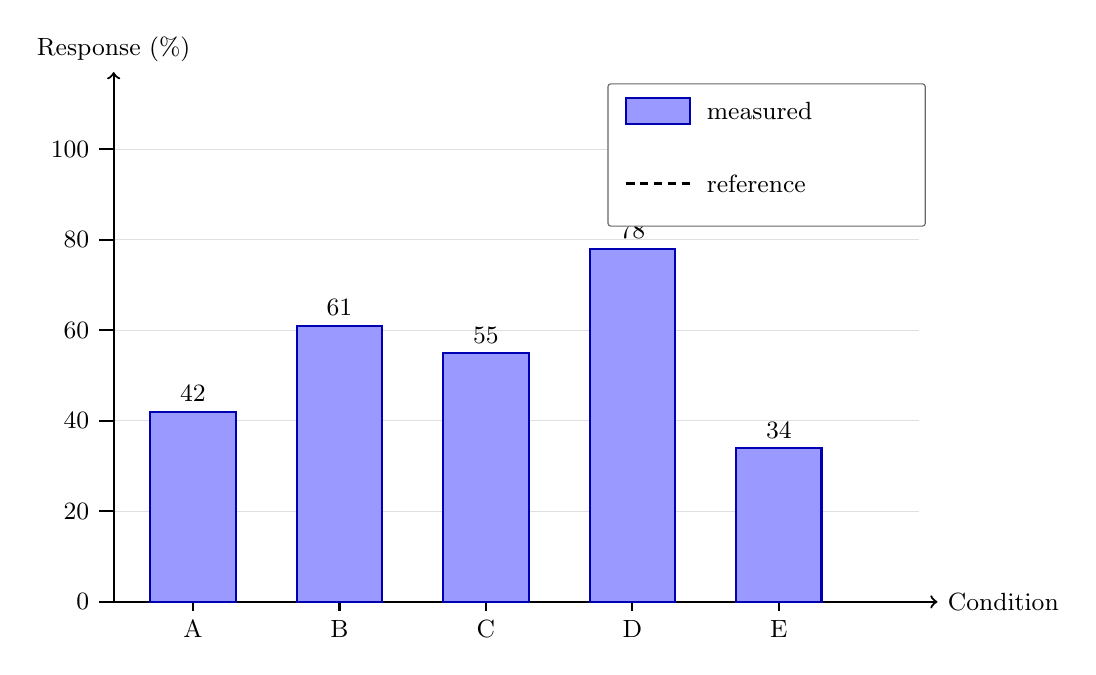
\begin{tikzpicture}[x=1.55cm, y=1.15cm, font=\small]

  % ---------------- grid ----------------
  \foreach \y in {1,2,3,4,5}{%
    \draw[gray!25, very thin] (0,\y) -- (6.6,\y);
  }

  % ---------------- axes ----------------
  \draw[->, thick] (0,0) -- (6.75,0) node[right, font=\small] {Condition};
  \draw[->, thick] (0,0) -- (0,5.85) node[above, font=\small] {Response (\%)};

  % x ticks + labels
  \foreach \x/\lab in {0.65/A, 1.85/B, 3.05/C, 4.25/D, 5.45/E}{%
    \draw[thick] (\x,0) -- (\x,-0.10);
    \node[below, font=\small] at (\x,-0.10) {\lab};
  }
  % y ticks + numeric labels
  \foreach \y/\lab in {0/0, 1/20, 2/40, 3/60, 4/80, 5/100}{%
    \draw[thick] (0,\y) -- (-0.12,\y);
    \node[left, font=\small] at (-0.12,\y) {\lab};
  }

  % ---------------- bars ----------------
  \foreach \x/\h/\v in {0.3/2.10/42, 1.5/3.05/61, 2.7/2.75/55, 3.9/3.90/78, 5.1/1.70/34}{%
    \draw[fill=blue!40, draw=blue!70!black, thick]
      (\x,0) rectangle (\x+0.7,\h);
    \node[above, font=\small] at (\x+0.35,\h) {\v};
  }

  % ---------------- legend ----------------
  \draw[draw=black!60, fill=white, rounded corners=1pt]
        (4.05,4.15) rectangle (6.65,5.72);
  \draw[fill=blue!40, draw=blue!70!black, thick]
        (4.20,5.28) rectangle (4.72,5.56);
  \node[right, font=\small] at (4.78,5.42) {measured};
  \draw[draw=black, thick, densely dashed] (4.20,4.62) -- (4.72,4.62);
  \node[right, font=\small] at (4.78,4.62) {reference};

\end{tikzpicture}
\end{document}
